\documentclass[12pt]{article}
\usepackage{amsmath,amssymb,amsthm}
\usepackage{graphicx,mathabx}
\usepackage{xcolor}
\usepackage{tikz}
\usepackage{placeins}
\usepackage{lipsum}
\usepackage[shortlabels]{enumitem}
\usepackage{placeins}
\usepackage[makeroom]{cancel}
\usepackage[strings]{underscore} 
\usepackage{afterpage}
\newcommand\tab[1][1cm]{\hspace*{#1}}
\newcommand\blankpage{%
    \null
    \thispagestyle{empty}%
    \addtocounter{page}{-1}%
    \newpage}
\begin{document}
\title{TCSS 343 - Week 5}
\author{Jake McKenzie}
\maketitle
\noindent\centerline{\textbf{Dynamic Programming}}\\\\\\\\\\\\
\begin{center}
    ``Perhaps thinking should be measured not by what you do \\but by how you do it." \\$\dots$\\ Richard Hamming
\end{center}
\begin{center}
    ``For the last sixty five years(speaking in 2018), due to Moore's law, with a clockwork precision, computer capability has been doubling every year and a half. Without fast algorithms you cannot bring to bare Moore's Law. A dramatic increase in computer speed needs to be coupled with efficient algorithms." \\$\dots$\\ Christos Papadimitriou
\end{center}
\begin{center}
    ``Nobody expects plumbers to have a physics degree but they do have to know some things about water physics, and that can be learned in a way that doesn’t necessarily involve getting a physics degree. And that is super cool, totally valid, and not a problem. But that doesn’t mean that physics degrees are bullshit or not useful to plumbers." \\$\dots$\\ Steve Klabnik \\(analogy on studying CS theory as a programmer)
\end{center}
\newpage
\noindent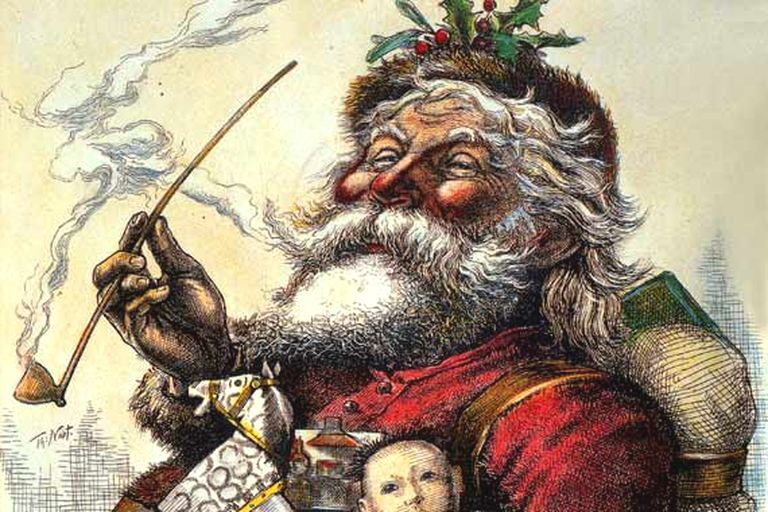
\includegraphics[scale = .32]{santa.jpg}\\
\noindent 1. Suppose Santa has 6 kinds of toys, each kind of toy has its own weight $w_i$ in tons, happiness rating $h_i$ in ... joy, and quantity $n_i$. Santa would like to maximize the total hapiness of the children but the total weight of his bag cannot exceed 17 tons. Their weight, hapiness rating and quantity are defined above. Please help Santa by filling in the DP table below, where dp[i][j] indicates the maximum value you can get with weight less or equal to $j$ using toys 1 to $i$. What is the final solution to this problem and briefly explain how you came to this solution. To help you get started, $23$ was generated by solving the equation $i_1+2i_2+3i_3 \leq 15$ which gives you the most value. That value was found by $3\cdot 1+ 2 \cdot 4 + 2 \cdot 6 = 23$. $12$ was found by solving the equation $i_1+2i_2+3i_3+4i_4+5i_5+6i_6 \leq 6$ which gives you the most value. That value was found by $2\cdot 6 = 12$ 
\begin{table}[]
\begin{tabular}{|l|l|l|l|}
\hline
i & $w_i$ & $h_i$ & $n_i$ \\ \hline
1 & 1    & 1    & 3    \\ \hline
2 & 2    & 4    & 2    \\ \hline
3 & 3    & 6    & 2    \\ \hline
4 & 4    & 5    & 1    \\ \hline
5 & 5    & 7    & 1    \\ \hline
6 & 6    & 8    & 1    \\ \hline
\end{tabular}
\end{table}
\FloatBarrier
\begin{table}[]
    \begin{tabular}{|l|l|l|l|l|l|l|l|l|l|l|l|l|l|l|l|l|l|l|}
    \hline
    i\textbackslash{}w & 0 & 1 & 2 & 3 & 4 & 5 & 6  & 7 & 8 & 9 & 10 & 11 & 12 & 13 & 14 & 15 & 16 & 17 \\ \hline
    \{1\}                  & 0 &   &   &   &   &   &    &   &   &   &    &    &    &    &    &    &    &    \\ \hline
    \{1,2\}                  & 0 &   &   &   &   &   &    &   &   &   &    &    &    &    &    &    &    &    \\ \hline
    \{1,2,3\}                  & 0 &   &   &   &   &   &    &   &   &   &    &    &    &    &    & 23 &    &    \\ \hline
    \{1,2,3,4\}                  & 0 &   &   &   &   &   &    &   &   &   &    &    &    &    &    &    &    &    \\ \hline
    \{1,2,3,4,5\}                  & 0 &   &   &   &   &   &    &   &   &   &    &    &    &    &    &    &    &    \\ \hline
    \{1,2,3,4,5,6\}                  & 0 &   &   &   &   &   & 12 &   &   &   &    &    &    &    &    &    &    &    \\ \hline
    \end{tabular}
    \end{table}
\newpage
\noindent 2. For much of this worksheet we will explore the ``placing parenthesis" problem. First
I want you to compute the maximum value of the expression given that you can placeins
a parenthesis between any two pair of numbers:\\
$$1+2-3 \times 4-5$$
(example of one possible ordering of parenthesis:$((((1+2)-3) \times 4)-5)=-5$)\\\\\\\\\\\\\\\\\\\\\\\\
3. How many different ordering of arithmetic operations are there in this problem? 
Why do we care about solving this problem with dynamic programming(find runtime of brute force)?\\\\\\\\\\\\\\\\\\\\\\\\
4. How many possible orderings are there for the expression: $$5-8+7 \times 4 - 8 + 9$$ 
(do not attempt to solve for the maximum possible ordering just yet!)
\newpage
\noindent \textbf{Placing Parentheses:}\\
\textbf{Input:} A sequence of digits $d_1$,$\dots$,$d_n$ and a sequence of operations $op_1$,$\dots$,$op_{n-1} \in \{ +,-,\times \}$.\\
\textbf{Output:} An order of applying these operations that maximizes the value of the expression.\\\\
\textbf{INTUITION:} Assume that the last operation in an optimal parenthesizing 
is when multiplication is done last, which with our previous example limits our possible
perumtations to the including this parenthesization:
$$(5-8+7) \times (4 - 8 + 9)$$
5. Now above, we've gone from having $5!$ possible
permutations of orderings to now having $2! + 2!$ possible orderings
because we've reduced our global problem into two more managable subproblems
by taking advantage of the shape of the problem. You may not understand why yet, but find each
parenthesization that maximizes and minimizes the following subproblems:\\\\
$min\{5-8+7\}=$\\
$max\{5-8+7\}=$\\
$min\{4-8+9\}=$\\
$max\{4-8+9\}=$\\\\
6. Using what you've found 
find the maximum value of the given expression below
and it's parenthesization:\\\\
$max\{(5-8+7) \times (4-8+9)\}=$\\\\
7. Why can't we be greedy and choose the maximum value at each stage? 
\newpage
\noindent Let $E_{ij}$ be the subexpression
$$d_i op_i \dots op_{j-1}d_j$$
Where are subproblems are defined as:
$$M(i,j) = \text{maximum value of } E_{ij}$$
$$m(i,j) = \text{minimum value of } E_{ij}$$
8. Given the information above and what you did on the prior page, 
can you write down a recurrence relation that solves the placing 
parenthesis problem? (HINT: remember that there are $2! + 2!$ possible 
orderings now that we usered our intuition! Both $M$ and $m$ will
have at least $4$ possible orderings each)\\\\\\\\\\\\\\\\\\
9. What do we mean when we say: `` Our current relation expresses 
the solution for an expression (i,j) for a solution for smaller 
sub subexpressions"?\\\\\\\\\\\\
A. When computing $M(i,j)$ the values of _______________ 
should already be computed.
\begin{enumerate}[a)]
    \item $M(i,k)$ and $M(k+1,j)$
    \item $M(i-1,k)$ and  $M(i,k-1)$
    \item $M(\frac{i}{2},k)$ and  $M(i,\frac{k}{2})$
\end{enumerate}
B. We need to solve all subproblems in order of ______________.
\begin{enumerate}[a)]
    \item decreasing $(j-i)$
    \item increasing $(j-i)$
\end{enumerate}
\newpage
\noindent C. For this algorithm we have roughly ____________ number of subproblems. 
\begin{enumerate}[a)]
    \item Linear
    \item Quadratic
    \item Exponential
    \item Tetratic
\end{enumerate}
Below I will give you the algorithm to compute the parenthesis problem.
I didn't ask you to construct it because it is quite complicated, I am 
much more interested in you seeing what it look like having explored the problem
suffiecently up to this point. Before you move on: \textbf{Make sure you
understand what each and every line is doing.} Please ask questions if you
have them. This is as important as answering the questions.\\
\noindent \textbf{MinAndMax(i,j):}\\
$min \leftarrow +\infty$\\
$max \leftarrow -\infty$\\
for $k$ from $i$ to $j-1$:\\
$\tab a \leftarrow M(i,k)$ $op_k$ $M(k+1,j)$\\
$\tab b \leftarrow m(i,k)$ $op_k$ $M(k+1,j)$\\
$\tab c \leftarrow M(i,k)$ $op_k$ $M(k+1,j)$\\
$\tab d \leftarrow m(i,k)$ $op_k$ $M(k+1,j)$\\
$\tab min \leftarrow min\{min,a,b,c,d\}$\\
$\tab max \leftarrow min\{max,a,b,c,d\}$\\
return $(min,max)$\\
\noindent \textbf{Parentheses($d_1 op_1$, $d_2 op_2$, $\dots$, $d_n op_n$):}\\
for $i$ from $1$ to $n$:\\
$\tab m(i,i) \leftarrow d_i$, $M(i,i)\leftarrow d_i$
for $s$ from $1$ to $n-1$:\\
$\tab$ for $s$ from $1$ to $n-s$:\\
$\tab\tab$ $j \leftarrow i+s$\\
$\tab\tab$ $m(i,j),M(i,j) \leftarrow MinAndMax(i,j)$\\
return $M(1,n)$\\\\
D. What is the worstcase runtime of the \textbf{Parentheses} algorithm above? (HINT: What is $j-i$ at most?)
\newpage
\noindent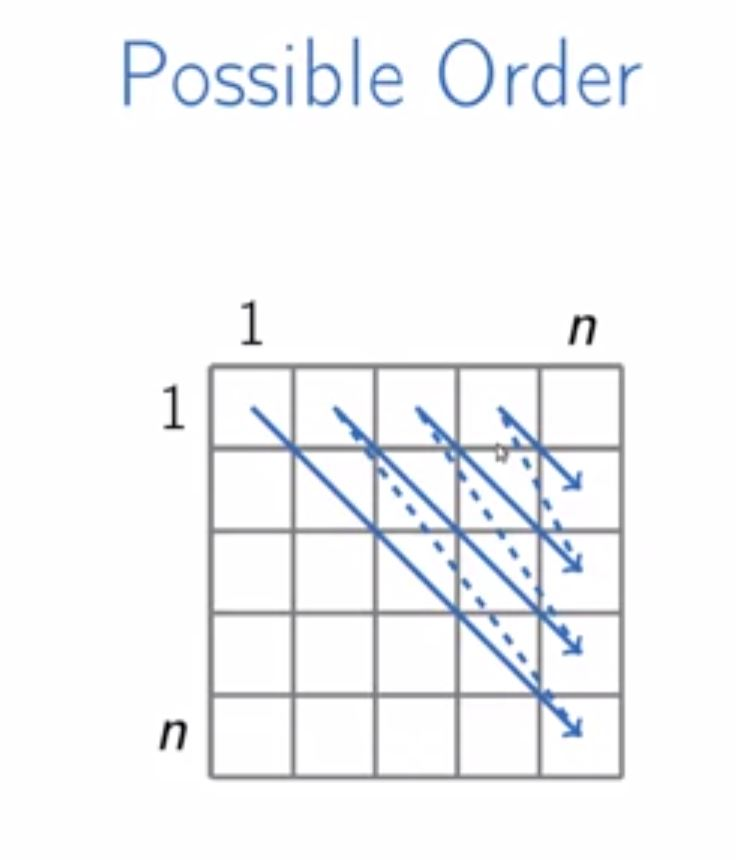
\includegraphics[scale = .3]{order.jpg}\\
Above is the possible ordering of how the algorithm 
stores the results of $m$ and $M$ where $i$ is 
row-wise and $j$ is column-wise.\\\\
Down each diagonal will be filled with each value of the arithmetic expression.\\
E. I will now ask you, using the algorithm stated previously, 
to constrcut the table produced by the algorithm. I was kind and gave you
two of the values in each of the tables to help you along. (HINT to get started:
can you break down the subexpression $5-8$ any further?)\\\\
Reminder of the expression we're maximizing:
$5-8+7 \times 4-8+9$
\FloatBarrier
\begin{table}[]
    \begin{tabular}{llllllllllllllll}
    m                      &                        &                        &                          &                        &                        &                        &  &  & M                      &                        &                        &                        &                        &                        &                        \\
    i\textbackslash{}j     & 1                      &                        &                          &                        &                        & n                      &  &  & i\textbackslash{}j     & 1                      &                        &                        &                        &                        & n                      \\ \cline{2-7} \cline{11-16} 
    \multicolumn{1}{l|}{1} & \multicolumn{1}{l|}{5} & \multicolumn{1}{l|}{}  & \multicolumn{1}{l|}{-10} & \multicolumn{1}{l|}{}  & \multicolumn{1}{l|}{}  & \multicolumn{1}{l|}{}  &  &  & \multicolumn{1}{l|}{1} & \multicolumn{1}{l|}{5} & \multicolumn{1}{l|}{}  & \multicolumn{1}{l|}{}  & \multicolumn{1}{l|}{}  & \multicolumn{1}{l|}{}  & \multicolumn{1}{l|}{}  \\ \cline{2-7} \cline{11-16} 
    \multicolumn{1}{l|}{}  & \multicolumn{1}{l|}{}  & \multicolumn{1}{l|}{8} & \multicolumn{1}{l|}{}    & \multicolumn{1}{l|}{}  & \multicolumn{1}{l|}{}  & \multicolumn{1}{l|}{}  &  &  & \multicolumn{1}{l|}{}  & \multicolumn{1}{l|}{}  & \multicolumn{1}{l|}{8} & \multicolumn{1}{l|}{}  & \multicolumn{1}{l|}{}  & \multicolumn{1}{l|}{}  & \multicolumn{1}{l|}{}  \\ \cline{2-7} \cline{11-16} 
    \multicolumn{1}{l|}{}  & \multicolumn{1}{l|}{}  & \multicolumn{1}{l|}{}  & \multicolumn{1}{l|}{7}   & \multicolumn{1}{l|}{}  & \multicolumn{1}{l|}{}  & \multicolumn{1}{l|}{}  &  &  & \multicolumn{1}{l|}{}  & \multicolumn{1}{l|}{}  & \multicolumn{1}{l|}{}  & \multicolumn{1}{l|}{7} & \multicolumn{1}{l|}{}  & \multicolumn{1}{l|}{}  & \multicolumn{1}{l|}{}  \\ \cline{2-7} \cline{11-16} 
    \multicolumn{1}{l|}{}  & \multicolumn{1}{l|}{}  & \multicolumn{1}{l|}{}  & \multicolumn{1}{l|}{}    & \multicolumn{1}{l|}{4} & \multicolumn{1}{l|}{}  & \multicolumn{1}{l|}{}  &  &  & \multicolumn{1}{l|}{}  & \multicolumn{1}{l|}{}  & \multicolumn{1}{l|}{}  & \multicolumn{1}{l|}{}  & \multicolumn{1}{l|}{4} & \multicolumn{1}{l|}{}  & \multicolumn{1}{l|}{5} \\ \cline{2-7} \cline{11-16} 
    \multicolumn{1}{l|}{}  & \multicolumn{1}{l|}{}  & \multicolumn{1}{l|}{}  & \multicolumn{1}{l|}{}    & \multicolumn{1}{l|}{}  & \multicolumn{1}{l|}{8} & \multicolumn{1}{l|}{}  &  &  & \multicolumn{1}{l|}{}  & \multicolumn{1}{l|}{}  & \multicolumn{1}{l|}{}  & \multicolumn{1}{l|}{}  & \multicolumn{1}{l|}{}  & \multicolumn{1}{l|}{8} & \multicolumn{1}{l|}{}  \\ \cline{2-7} \cline{11-16} 
    \multicolumn{1}{l|}{n} & \multicolumn{1}{l|}{}  & \multicolumn{1}{l|}{}  & \multicolumn{1}{l|}{}    & \multicolumn{1}{l|}{}  & \multicolumn{1}{l|}{}  & \multicolumn{1}{l|}{9} &  &  & \multicolumn{1}{l|}{n} & \multicolumn{1}{l|}{}  & \multicolumn{1}{l|}{}  & \multicolumn{1}{l|}{}  & \multicolumn{1}{l|}{}  & \multicolumn{1}{l|}{}  & \multicolumn{1}{l|}{9} \\ \cline{2-7} \cline{11-16} 
    \end{tabular}
    \end{table}
    \FloatBarrier
\newpage
\noindent F. How would you use the table to reconstruct the solution? I know that at this
point you probably know the optimal subexpression is but we must think algorithmically
so that we can tell the dumbest thing on the planet, namely a computer, how to
do it. Sorry I ran out of space on the last page. Please try to trace the steps in the matrix
and think about how you would reconstruct the solution by stepping forward and backward that got you
to $M(6,6)$. Can you write that expression as an ordering of $m$ and $M$ ordered pairs?\\\\
\newpage
\noindent The longest common subsequcne can be broken donw to two cases, given two strings represented as character arrays:\\\\
\textbf{Case 1: } If $S_1[i]\cancel{=}S_2[j]$ then we have that: $$LCS(i,j)=Max\{LCS(i-1,j),LCS(i,j-1)\}$$\\\\
\textbf{Case 2: } If $S_1[i]=S_2[j]$ then we have that: $$LCS(i,j)=1+ LCS(i-1,j-1)$$
10. Using your notes or the information I just provided to fill out the rest of this table.
\FloatBarrier
\begin{table}[]
    \begin{tabular}{lllllll}
                           & B                      & A                      & C                     & B                     & A                      & D                     \\ \cline{2-7} 
    \multicolumn{1}{l|}{A} & \multicolumn{1}{l|}{0} & \multicolumn{1}{l|}{}  & \multicolumn{1}{l|}{} & \multicolumn{1}{l|}{} & \multicolumn{1}{l|}{}  & \multicolumn{1}{l|}{} \\ \cline{2-7} 
    \multicolumn{1}{l|}{B} & \multicolumn{1}{l|}{}  & \multicolumn{1}{l|}{}  & \multicolumn{1}{l|}{} & \multicolumn{1}{l|}{} & \multicolumn{1}{l|}{}  & \multicolumn{1}{l|}{} \\ \cline{2-7} 
    \multicolumn{1}{l|}{A} & \multicolumn{1}{l|}{}  & \multicolumn{1}{l|}{2} & \multicolumn{1}{l|}{} & \multicolumn{1}{l|}{} & \multicolumn{1}{l|}{}  & \multicolumn{1}{l|}{} \\ \cline{2-7} 
    \multicolumn{1}{l|}{Z} & \multicolumn{1}{l|}{}  & \multicolumn{1}{l|}{}  & \multicolumn{1}{l|}{} & \multicolumn{1}{l|}{} & \multicolumn{1}{l|}{}  & \multicolumn{1}{l|}{} \\ \cline{2-7} 
    \multicolumn{1}{l|}{D} & \multicolumn{1}{l|}{}  & \multicolumn{1}{l|}{}  & \multicolumn{1}{l|}{} & \multicolumn{1}{l|}{} & \multicolumn{1}{l|}{3} & \multicolumn{1}{l|}{} \\ \cline{2-7} 
    \multicolumn{1}{l|}{C} & \multicolumn{1}{l|}{}  & \multicolumn{1}{l|}{}  & \multicolumn{1}{l|}{} & \multicolumn{1}{l|}{} & \multicolumn{1}{l|}{}  & \multicolumn{1}{l|}{} \\ \cline{2-7} 
    \end{tabular}
    \end{table}
    \FloatBarrier
\noindent \textbf{Dance Dance Revolution} n is a dance video game, 
first introduced in Japan by Konami in
1998. Players stand on a platform marked 
with four arrows, pointing forward, back, left,
and right, arranged in a cross pattern. 
During play, the game plays a song and scrolls a
sequence of n arrows ($\leftarrow$, $\uparrow$,$\downarrow$, or $\rightarrow$) from the 
bottom to the top of the screen. At the
precise moment each arrow reaches the top of the 
screen, the player must step on the
corresponding arrow on the dance platform. (The 
arrows are timed so that you’ll step with
the beat of the song.)\\\\
You are playing a variant of this game called ``Vogue Vogue Revolution", where the goal
is to play perfectly but move as little as possible. When an arrow reaches the top of the
screen, if one of your feet is already on the correct arrow, you are awarded one style point
for maintaining your current pose. If neither foot is on the right arrow, you must move one
(and only one) of your feet from its current location to the correct arrow on the platform.
If you ever step on the wrong arrow, or fail to step on the correct arrow, or move more
than one foot at a time, or move either foot when you are already standing on the correct
arrow, all your style points are taken away and you lose the game.\\\\
How should you move your feet to maximize your total number of style points? For
purposes of this problem, assume you always start with you left foot on $\leftarrow$
and you right
foot on $\rightarrow$, and that you’ve memorized the entire sequence of arrows. For example, if the
sequence is $\uparrow\uparrow\downarrow\downarrow\leftarrow\rightarrow\leftarrow\rightarrow$, you can earn $5$ style points by moving you feet as shown
below:\\\\
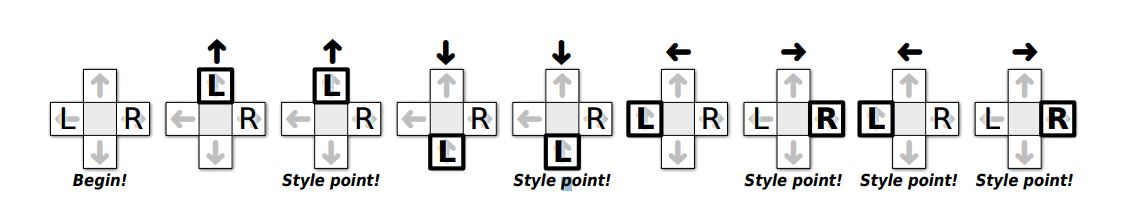
\includegraphics[width=\textwidth]{ddr.jpg}\\
11. Prove that for any sequence of n arrows, it is possible to earn at least $\frac{n}{4} - 1$ style
points.\\\\\
12. Describe an efficient algorithm to find the maximum number of style points you can
earn during a given VVR routine. The input to your algorithm is an array $Arrow[1 \dots n]$
containing the sequence of arrows.
\afterpage{\blankpage}
\newpage
\noindent 13. In mathematics, a sequence of positive real numbers 
$s_1$, $s_2$,$\dots$ is called \textit{superincreasing} if each element
in the sequence is greater than the sum of all previous elements in the sequence:
$$s_{n+1} > \sum\limits_{i=1}^{n}s_i$$
For example: \{$2,3,7,16,65,321,4546$\} is a superincreasing sequence, 
but \{$1,1,2,5,15,52,203,877$\} us not a superincreasing sequence.\\\\
Describe an algorithm that takes as input superincreasing sequence $s_1,\dots,s_n$ and a positive 
integer $k$, please find a sequnce of $s_1,\dots,s_n$ with the sum equal
to $k$. It is possible and desirable to find an algorithm that can accomplish this
task in $O(n)$ time using dynamic progrmaming. If you think you've come up with an
algorithm that can accomplish this task attempt to prove that it is correct.
\newpage
\noindent A \textit{covering} or \textit{vertex cover} of a graph $G$ is a subset $U ⊆ V(G)$ that covers every
edge of $G$; that is, every edge has at least one endpoint in $U$. The white dots below
in the following graphs are \textit{coverings} of G.\\\\
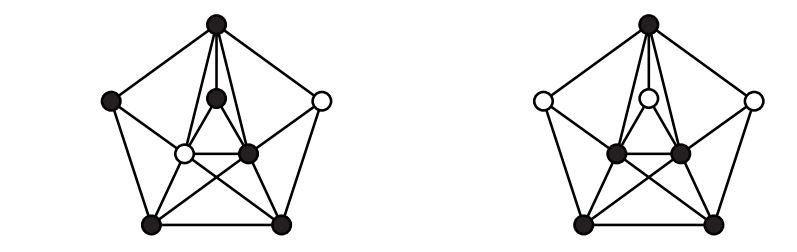
\includegraphics[width=\textwidth]{covering.jpg}\\
14. For the following graphs find a minimum \textit{covering} of the graph(there may
be more than one minimum covering for the graph).\\
\centerline{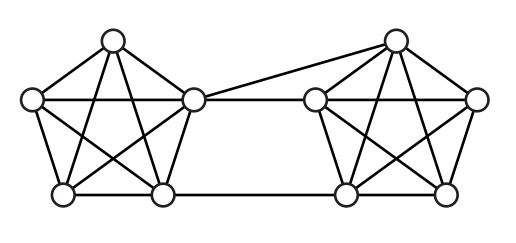
\includegraphics[scale=0.5]{graph2.jpg}}\\
\centerline{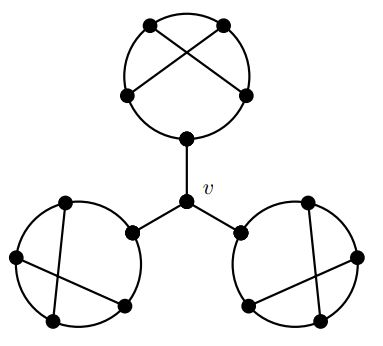
\includegraphics[scale=0.5]{graph1.jpg}}\\
15. Computing the \textit{covering} is an NP-Complete problem, even when we approximate the solution. 
If you haven't covered this yet in class that's okay.
To put simply for now, NP-Complete problems are ones we know are \textbf{hard}.\\
Think about how you you go about finding the \textit{covering}. You don't have to give psuedocode,
but I do suggest talking amongst your peers to how you would go about coming up with an algorithm
to compute the \textit{covering}.
\newpage
\end{document}